% Options for packages loaded elsewhere
\PassOptionsToPackage{unicode}{hyperref}
\PassOptionsToPackage{hyphens}{url}
%
\documentclass[
]{article}
\usepackage{amsmath,amssymb}
\usepackage{iftex}
\ifPDFTeX
  \usepackage[T1]{fontenc}
  \usepackage[utf8]{inputenc}
  \usepackage{textcomp} % provide euro and other symbols
\else % if luatex or xetex
  \usepackage{unicode-math} % this also loads fontspec
  \defaultfontfeatures{Scale=MatchLowercase}
  \defaultfontfeatures[\rmfamily]{Ligatures=TeX,Scale=1}
\fi
\usepackage{lmodern}
\ifPDFTeX\else
  % xetex/luatex font selection
\fi
% Use upquote if available, for straight quotes in verbatim environments
\IfFileExists{upquote.sty}{\usepackage{upquote}}{}
\IfFileExists{microtype.sty}{% use microtype if available
  \usepackage[]{microtype}
  \UseMicrotypeSet[protrusion]{basicmath} % disable protrusion for tt fonts
}{}
\makeatletter
\@ifundefined{KOMAClassName}{% if non-KOMA class
  \IfFileExists{parskip.sty}{%
    \usepackage{parskip}
  }{% else
    \setlength{\parindent}{0pt}
    \setlength{\parskip}{6pt plus 2pt minus 1pt}}
}{% if KOMA class
  \KOMAoptions{parskip=half}}
\makeatother
\usepackage{xcolor}
\usepackage[margin=1in]{geometry}
\usepackage{color}
\usepackage{fancyvrb}
\newcommand{\VerbBar}{|}
\newcommand{\VERB}{\Verb[commandchars=\\\{\}]}
\DefineVerbatimEnvironment{Highlighting}{Verbatim}{commandchars=\\\{\}}
% Add ',fontsize=\small' for more characters per line
\usepackage{framed}
\definecolor{shadecolor}{RGB}{248,248,248}
\newenvironment{Shaded}{\begin{snugshade}}{\end{snugshade}}
\newcommand{\AlertTok}[1]{\textcolor[rgb]{0.94,0.16,0.16}{#1}}
\newcommand{\AnnotationTok}[1]{\textcolor[rgb]{0.56,0.35,0.01}{\textbf{\textit{#1}}}}
\newcommand{\AttributeTok}[1]{\textcolor[rgb]{0.13,0.29,0.53}{#1}}
\newcommand{\BaseNTok}[1]{\textcolor[rgb]{0.00,0.00,0.81}{#1}}
\newcommand{\BuiltInTok}[1]{#1}
\newcommand{\CharTok}[1]{\textcolor[rgb]{0.31,0.60,0.02}{#1}}
\newcommand{\CommentTok}[1]{\textcolor[rgb]{0.56,0.35,0.01}{\textit{#1}}}
\newcommand{\CommentVarTok}[1]{\textcolor[rgb]{0.56,0.35,0.01}{\textbf{\textit{#1}}}}
\newcommand{\ConstantTok}[1]{\textcolor[rgb]{0.56,0.35,0.01}{#1}}
\newcommand{\ControlFlowTok}[1]{\textcolor[rgb]{0.13,0.29,0.53}{\textbf{#1}}}
\newcommand{\DataTypeTok}[1]{\textcolor[rgb]{0.13,0.29,0.53}{#1}}
\newcommand{\DecValTok}[1]{\textcolor[rgb]{0.00,0.00,0.81}{#1}}
\newcommand{\DocumentationTok}[1]{\textcolor[rgb]{0.56,0.35,0.01}{\textbf{\textit{#1}}}}
\newcommand{\ErrorTok}[1]{\textcolor[rgb]{0.64,0.00,0.00}{\textbf{#1}}}
\newcommand{\ExtensionTok}[1]{#1}
\newcommand{\FloatTok}[1]{\textcolor[rgb]{0.00,0.00,0.81}{#1}}
\newcommand{\FunctionTok}[1]{\textcolor[rgb]{0.13,0.29,0.53}{\textbf{#1}}}
\newcommand{\ImportTok}[1]{#1}
\newcommand{\InformationTok}[1]{\textcolor[rgb]{0.56,0.35,0.01}{\textbf{\textit{#1}}}}
\newcommand{\KeywordTok}[1]{\textcolor[rgb]{0.13,0.29,0.53}{\textbf{#1}}}
\newcommand{\NormalTok}[1]{#1}
\newcommand{\OperatorTok}[1]{\textcolor[rgb]{0.81,0.36,0.00}{\textbf{#1}}}
\newcommand{\OtherTok}[1]{\textcolor[rgb]{0.56,0.35,0.01}{#1}}
\newcommand{\PreprocessorTok}[1]{\textcolor[rgb]{0.56,0.35,0.01}{\textit{#1}}}
\newcommand{\RegionMarkerTok}[1]{#1}
\newcommand{\SpecialCharTok}[1]{\textcolor[rgb]{0.81,0.36,0.00}{\textbf{#1}}}
\newcommand{\SpecialStringTok}[1]{\textcolor[rgb]{0.31,0.60,0.02}{#1}}
\newcommand{\StringTok}[1]{\textcolor[rgb]{0.31,0.60,0.02}{#1}}
\newcommand{\VariableTok}[1]{\textcolor[rgb]{0.00,0.00,0.00}{#1}}
\newcommand{\VerbatimStringTok}[1]{\textcolor[rgb]{0.31,0.60,0.02}{#1}}
\newcommand{\WarningTok}[1]{\textcolor[rgb]{0.56,0.35,0.01}{\textbf{\textit{#1}}}}
\usepackage{graphicx}
\makeatletter
\def\maxwidth{\ifdim\Gin@nat@width>\linewidth\linewidth\else\Gin@nat@width\fi}
\def\maxheight{\ifdim\Gin@nat@height>\textheight\textheight\else\Gin@nat@height\fi}
\makeatother
% Scale images if necessary, so that they will not overflow the page
% margins by default, and it is still possible to overwrite the defaults
% using explicit options in \includegraphics[width, height, ...]{}
\setkeys{Gin}{width=\maxwidth,height=\maxheight,keepaspectratio}
% Set default figure placement to htbp
\makeatletter
\def\fps@figure{htbp}
\makeatother
\setlength{\emergencystretch}{3em} % prevent overfull lines
\providecommand{\tightlist}{%
  \setlength{\itemsep}{0pt}\setlength{\parskip}{0pt}}
\setcounter{secnumdepth}{-\maxdimen} % remove section numbering
\ifLuaTeX
  \usepackage{selnolig}  % disable illegal ligatures
\fi
\IfFileExists{bookmark.sty}{\usepackage{bookmark}}{\usepackage{hyperref}}
\IfFileExists{xurl.sty}{\usepackage{xurl}}{} % add URL line breaks if available
\urlstyle{same}
\hypersetup{
  pdftitle={Reproduciblity: Bayesian Regression for Directional Data},
  hidelinks,
  pdfcreator={LaTeX via pandoc}}

\title{Reproduciblity: Bayesian Regression for Directional Data}
\author{}
\date{\vspace{-2.5em}}

\begin{document}
\maketitle

\hypertarget{loading-the-r-package}{%
\section{Loading the R Package}\label{loading-the-r-package}}

\begin{Shaded}
\begin{Highlighting}[]
\FunctionTok{library}\NormalTok{(RBVNF)}
\end{Highlighting}
\end{Shaded}

\begin{verbatim}
## 
## Attaching package: 'RBVNF'
\end{verbatim}

\begin{verbatim}
## The following object is masked from 'package:base':
## 
##     norm
\end{verbatim}

\begin{Shaded}
\begin{Highlighting}[]
\FunctionTok{load\_packages}\NormalTok{()}
\end{Highlighting}
\end{Shaded}

\begin{verbatim}
## Loading required package: numDeriv
\end{verbatim}

\begin{verbatim}
## Loading required package: MASS
\end{verbatim}

\begin{verbatim}
## Loading required package: Rcpp
\end{verbatim}

\begin{verbatim}
## Loading required package: RcppZiggurat
\end{verbatim}

\begin{verbatim}
## Loading required package: RcppParallel
\end{verbatim}

\begin{verbatim}
## 
## Attaching package: 'RcppParallel'
\end{verbatim}

\begin{verbatim}
## The following object is masked from 'package:Rcpp':
## 
##     LdFlags
\end{verbatim}

\begin{verbatim}
## 
## Rfast: 2.1.0
\end{verbatim}

\begin{verbatim}
##  ___ __ __ __ __    __ __ __ __ __ _             _               __ __ __ __ __     __ __ __ __ __ __   
## |  __ __ __ __  |  |  __ __ __ __ _/            / \             |  __ __ __ __ /   /__ __ _   _ __ __\  
## | |           | |  | |                         / _ \            | |                        / /          
## | |           | |  | |                        / / \ \           | |                       / /          
## | |           | |  | |                       / /   \ \          | |                      / /          
## | |__ __ __ __| |  | |__ __ __ __           / /     \ \         | |__ __ __ __ _        / /__/\          
## |    __ __ __ __|  |  __ __ __ __|         / /__ _ __\ \        |_ __ __ __ _   |      / ___  /           
## |   \              | |                    / _ _ _ _ _ _ \                     | |      \/  / /       
## | |\ \             | |                   / /           \ \                    | |         / /          
## | | \ \            | |                  / /             \ \                   | |        / /          
## | |  \ \           | |                 / /               \ \                  | |       / /          
## | |   \ \__ __ _   | |                / /                 \ \     _ __ __ __ _| |      / /          
## |_|    \__ __ __\  |_|               /_/                   \_\   /_ __ __ __ ___|      \/             team
\end{verbatim}

\begin{verbatim}
## Loading required package: cowplot
\end{verbatim}

\begin{verbatim}
## 
## Attaching package: 'mvtnorm'
\end{verbatim}

\begin{verbatim}
## The following objects are masked from 'package:Rfast':
## 
##     Crossprod, dmvnorm, dmvt, rmvnorm, rmvt, Tcrossprod
\end{verbatim}

\begin{verbatim}
## Loading required package: Matrix
\end{verbatim}

\begin{verbatim}
## Loaded glmnet 4.1-8
\end{verbatim}

\begin{Shaded}
\begin{Highlighting}[]
\FunctionTok{load\_additional\_packages}\NormalTok{()}
\end{Highlighting}
\end{Shaded}

\begin{verbatim}
## 
## Attaching package: 'plotly'
\end{verbatim}

\begin{verbatim}
## The following object is masked from 'package:ggplot2':
## 
##     last_plot
\end{verbatim}

\begin{verbatim}
## The following object is masked from 'package:MASS':
## 
##     select
\end{verbatim}

\begin{verbatim}
## The following object is masked from 'package:stats':
## 
##     filter
\end{verbatim}

\begin{verbatim}
## The following object is masked from 'package:graphics':
## 
##     layout
\end{verbatim}

\begin{verbatim}
## Loading required package: dplyr
\end{verbatim}

\begin{verbatim}
## 
## Attaching package: 'dplyr'
\end{verbatim}

\begin{verbatim}
## The following object is masked from 'package:gridExtra':
## 
##     combine
\end{verbatim}

\begin{verbatim}
## The following object is masked from 'package:Rfast':
## 
##     nth
\end{verbatim}

\begin{verbatim}
## The following object is masked from 'package:MASS':
## 
##     select
\end{verbatim}

\begin{verbatim}
## The following objects are masked from 'package:stats':
## 
##     filter, lag
\end{verbatim}

\begin{verbatim}
## The following objects are masked from 'package:base':
## 
##     intersect, setdiff, setequal, union
\end{verbatim}

\begin{verbatim}
## -- Attaching core tidyverse packages ------------------------ tidyverse 2.0.0 --
## v forcats   1.0.0     v stringr   1.5.0
## v lubridate 1.9.3     v tibble    3.2.1
## v purrr     1.0.2     v tidyr     1.3.0
## v readr     2.1.4     
## -- Conflicts ------------------------------------------ tidyverse_conflicts() --
## x dplyr::combine()    masks gridExtra::combine()
## x tidyr::expand()     masks Matrix::expand()
## x dplyr::filter()     masks plotly::filter(), stats::filter()
## x purrr::is_integer() masks Rfast::is_integer()
## x dplyr::lag()        masks stats::lag()
## x dplyr::nth()        masks Rfast::nth()
## x tidyr::pack()       masks Matrix::pack()
## x dplyr::select()     masks plotly::select(), MASS::select()
## x lubridate::stamp()  masks cowplot::stamp()
## x purrr::transpose()  masks Rfast::transpose()
## x tidyr::unpack()     masks Matrix::unpack()
## i Use the conflicted package (<http://conflicted.r-lib.org/>) to force all conflicts to become errors
\end{verbatim}

\hypertarget{simulated-data-generation-and-em-for-posterior-mode-d2-circular-data}{%
\subsection{Simulated Data Generation and EM for Posterior Mode (d=2,
Circular
Data):}\label{simulated-data-generation-and-em-for-posterior-mode-d2-circular-data}}

In this part of the demonstration, we generate a dataset of size n=750,
with p=10 (10 covariates) and the responses are circular,i.e., d=2. Then
we fit the EM algorithm to estimate the regression coefficients. True
value of the regression coefficients, and its estimates are printed.

\begin{Shaded}
\begin{Highlighting}[]
\NormalTok{n}\OtherTok{=}\DecValTok{750}  \CommentTok{\# NUmber of the samples}
\NormalTok{p}\OtherTok{=}\DecValTok{10}    \CommentTok{\# NUmber of the regression covariates}
\NormalTok{d}\OtherTok{=}\DecValTok{2}     \CommentTok{\# Number of direcions in the direcional data}
\DocumentationTok{\#\#\#\# bbeta is a matrix of dimension p\textbackslash{}times d}
\CommentTok{\#bbeta=matrix( rnorm(p*d), nrow=p, ncol=d)}
\NormalTok{sigma\_square}\OtherTok{=}\DecValTok{1}
\NormalTok{tau\_square}\OtherTok{=}\DecValTok{10000}
\NormalTok{data\_lst }\OtherTok{=} \FunctionTok{Data\_generator\_vnf\_reg}\NormalTok{(}\AttributeTok{n=}\NormalTok{n, }\AttributeTok{p=}\NormalTok{p, }\AttributeTok{d=}\NormalTok{d, }\AttributeTok{concentration\_factor =} \DecValTok{1}\NormalTok{, }\AttributeTok{beta\_factor =} \DecValTok{10}\NormalTok{)}
\NormalTok{Y }\OtherTok{=}\NormalTok{ data\_lst}\SpecialCharTok{$}\NormalTok{Y;X}\OtherTok{=}\NormalTok{data\_lst}\SpecialCharTok{$}\NormalTok{X;}

\CommentTok{\# Fitting the EM algorithm for the Standard Regresion for directional responses: This takes less than a minute. }
\NormalTok{beta\_EM}\OtherTok{=}\FunctionTok{EM\_Dir\_regression\_optimizer\_V1}\NormalTok{(}\AttributeTok{Y=}\NormalTok{Y, }\AttributeTok{X=}\NormalTok{X, }\AttributeTok{prior=}\ConstantTok{NULL}\NormalTok{, }\AttributeTok{beta\_init =} \ConstantTok{NULL}\NormalTok{,   }\AttributeTok{EM\_tolerence =}\NormalTok{ .}\DecValTok{00001}\NormalTok{)}
\end{Highlighting}
\end{Shaded}

\begin{verbatim}
## [1] 2
## [1] 3
## [1] 4
## [1] 5
## [1] 6
## [1] 7
## [1] 8
## [1] 9
## [1] 10
## [1] 11
## [1] 12
## [1] 13
## [1] 14
## [1] 15
## [1] 16
## [1] 17
## [1] 18
## [1] 19
## [1] 20
## [1] 21
## [1] 22
## [1] 23
## [1] 24
## [1] 25
## [1] 26
## [1] 27
## [1] 28
## [1] 29
## [1] 30
## [1] 31
## [1] 32
## [1] 33
## [1] 34
## [1] 35
## [1] 36
## [1] 37
## [1] 38
## [1] 39
## [1] 40
## [1] 41
## [1] 42
## [1] 43
## [1] 44
## [1] 45
## [1] 46
## [1] 47
## [1] 48
## [1] 49
## [1] 50
## [1] 51
## [1] 52
## [1] 53
## [1] 54
## [1] 55
## [1] 56
## [1] 57
## [1] 58
## [1] 59
## [1] 60
## [1] 61
## [1] 62
## [1] 63
## [1] 64
## [1] 65
## [1] 66
## [1] 67
## [1] 68
## [1] 69
## [1] 70
## [1] 71
## [1] 72
## [1] 73
## [1] 74
## [1] 75
## [1] 76
## [1] 77
## [1] 78
## [1] 79
## [1] 80
## [1] 81
## [1] 82
## [1] 83
## [1] 84
## [1] 85
## [1] 86
## [1] 87
## [1] 88
## [1] 89
## [1] 90
## [1] 91
## [1] 92
## [1] 93
## [1] 94
## [1] 95
## [1] 96
## [1] 97
## [1] 98
## [1] 99
## [1] 100
## [1] 101
## [1] 102
## [1] 103
## [1] 104
## [1] 105
## [1] 106
## [1] 107
## [1] 108
## [1] 109
## [1] 110
## [1] 111
## [1] 112
## [1] 113
## [1] 114
## [1] 115
## [1] 116
## [1] 117
## [1] 118
## [1] 119
## [1] 120
## [1] 121
## [1] 122
## [1] 123
## [1] 124
## [1] 125
## [1] 126
## [1] 127
## [1] 128
## [1] 129
## [1] 130
## [1] 131
## [1] 132
## [1] 133
## [1] 134
## [1] 135
## [1] 136
## [1] 137
## [1] 138
## [1] 139
## [1] 140
## [1] 141
## [1] 142
## [1] 143
## [1] 144
## [1] 145
## [1] 146
## [1] 147
## [1] 148
## [1] 149
## [1] 150
## [1] 151
## [1] 152
## [1] 153
## [1] 154
## [1] 155
## [1] 156
## [1] 157
## [1] 158
## [1] 159
## [1] 160
## [1] 161
## [1] 162
## [1] 163
## [1] 164
## [1] 165
## [1] 166
## [1] 167
## [1] 168
## [1] 169
## [1] 170
## [1] 171
## [1] 172
## [1] 173
## [1] 174
## [1] 175
## [1] 176
## [1] 177
## [1] 178
## [1] 179
## [1] 180
## [1] 181
## [1] 182
## [1] 183
## [1] 184
## [1] 185
## [1] 186
## [1] 187
## [1] 188
## [1] 189
## [1] 190
## [1] 191
## [1] 192
## [1] 193
## [1] 194
## [1] 195
## [1] 196
## [1] 197
## [1] 198
## [1] 199
## [1] 200
## [1] 201
## [1] 202
## [1] 203
## [1] 204
## [1] 205
## [1] 206
## [1] 207
## [1] 208
## [1] 209
## [1] 210
## [1] 211
## [1] 212
## [1] 213
## [1] 214
## [1] 215
## [1] 216
## [1] 217
## [1] 218
## [1] 219
## [1] 220
## [1] 221
## [1] 222
## [1] 223
## [1] 224
## [1] 225
## [1] 226
## [1] 227
## [1] 228
## [1] 229
## [1] 230
## [1] 231
## [1] 232
## [1] 233
## [1] 234
## [1] 235
## [1] 236
## [1] 237
## [1] 238
## [1] 239
## [1] 240
## [1] 241
## [1] 242
## [1] 243
## [1] 244
## [1] 245
## [1] 246
## [1] 247
## [1] 248
## [1] 249
## [1] 250
## [1] 251
## [1] 252
## [1] 253
## [1] 254
## [1] 255
## [1] 256
## [1] 257
## [1] 258
## [1] 259
## [1] 260
## [1] 261
## [1] 262
## [1] 263
## [1] 264
## [1] 265
## [1] 266
## [1] 267
## [1] 268
## [1] 269
## [1] 270
## [1] 271
## [1] 272
## [1] 273
## [1] 274
## [1] 275
## [1] 276
## [1] 277
## [1] 278
## [1] 279
## [1] 280
## [1] 281
## [1] 282
## [1] 283
## [1] 284
## [1] 285
## [1] 286
## [1] 287
## [1] 288
## [1] 289
## [1] 290
## [1] 291
## [1] 292
## [1] 293
## [1] 294
## [1] 295
## [1] 296
## [1] 297
## [1] 298
## [1] 299
## [1] 300
## [1] 301
## [1] 302
## [1] 303
## [1] 304
## [1] 305
## [1] 306
## [1] 307
## [1] 308
## [1] 309
## [1] 310
## [1] 311
## [1] 312
## [1] 313
## [1] 314
## [1] 315
## [1] 316
## [1] 317
## [1] 318
## [1] 319
## [1] 320
## [1] 321
## [1] 322
## [1] 323
## [1] 324
## [1] 325
## [1] 326
## [1] 327
## [1] 328
## [1] 329
## [1] 330
## [1] 331
## [1] 332
## [1] 333
## [1] 334
## [1] 335
## [1] 336
## [1] 337
## [1] 338
## [1] 339
## [1] 340
## [1] 341
## [1] 342
## [1] 343
## [1] 344
## [1] 345
## [1] 346
## [1] 347
## [1] 348
## [1] 349
## [1] 350
## [1] 351
## [1] 352
## [1] 353
## [1] 354
## [1] 355
## [1] 356
## [1] 357
## [1] 358
## [1] 359
## [1] 360
## [1] 361
## [1] 362
## [1] 363
## [1] 364
## [1] 365
## [1] 366
## [1] 367
## [1] 368
## [1] 369
## [1] 370
## [1] 371
## [1] 372
## [1] 373
## [1] 374
## [1] 375
## [1] 376
## [1] 377
## [1] 378
## [1] 379
## [1] 380
## [1] 381
## [1] 382
## [1] 383
## [1] 384
## [1] 385
## [1] 386
## [1] 387
## [1] 388
## [1] 389
## [1] 390
## [1] 391
## [1] 392
## [1] 393
## [1] 394
## [1] 395
## [1] 396
## [1] 397
## [1] 398
## [1] 399
## [1] 400
## [1] 401
## [1] 402
## [1] 403
## [1] 404
## [1] 405
## [1] 406
## [1] 407
## [1] 408
## [1] 409
## [1] 410
## [1] 411
## [1] 412
## [1] 413
## [1] 414
## [1] 415
## [1] 416
## [1] 417
## [1] 418
## [1] 419
## [1] 420
## [1] 421
## [1] 422
## [1] 423
## [1] 424
## [1] 425
## [1] 426
## [1] 427
## [1] 428
## [1] 429
## [1] 430
## [1] 431
## [1] 432
## [1] 433
## [1] 434
## [1] 435
## [1] 436
## [1] 437
## [1] 438
## [1] 439
## [1] 440
## [1] 441
## [1] 442
## [1] 443
## [1] 444
## [1] 445
## [1] 446
## [1] 447
## [1] 448
\end{verbatim}

\begin{Shaded}
\begin{Highlighting}[]
\FunctionTok{colnames}\NormalTok{(beta\_EM)}\OtherTok{=} \FunctionTok{gsub}\NormalTok{(}\StringTok{"Y"}\NormalTok{,}\StringTok{"Beta"}\NormalTok{, }\FunctionTok{colnames}\NormalTok{(beta\_EM))}
\FunctionTok{print}\NormalTok{(}\StringTok{"Estimated Beta="}\NormalTok{, beta\_EM)}
\end{Highlighting}
\end{Shaded}

\begin{verbatim}
## [1] "Estimated Beta="
\end{verbatim}

\begin{Shaded}
\begin{Highlighting}[]
\FunctionTok{print}\NormalTok{(}\FunctionTok{cbind}\NormalTok{(}\AttributeTok{EstimatedValue=}\FunctionTok{c}\NormalTok{(}\FunctionTok{t}\NormalTok{(beta\_EM)),}\AttributeTok{TrueValue=}\FunctionTok{c}\NormalTok{(}\FunctionTok{t}\NormalTok{(data\_lst}\SpecialCharTok{$}\NormalTok{beta))))}
\end{Highlighting}
\end{Shaded}

\begin{verbatim}
##       EstimatedValue  TrueValue
##  [1,]      9.4603965  9.1780961
##  [2,]      8.3957160  8.6681013
##  [3,]     -0.7941676 -0.6367181
##  [4,]      0.9737279  1.0669862
##  [5,]     -1.1275878 -0.9401547
##  [6,]      2.9266152  3.1512520
##  [7,]    -10.3556491 -9.9057587
##  [8,]      8.0430501  7.6063437
##  [9,]      7.1787617  7.4608627
## [10,]      2.4230743  2.7716209
## [11,]      3.4724951  3.5646314
## [12,]      6.8901778  6.9443400
## [13,]      1.9439854  1.6829277
## [14,]     -4.7436497 -4.7351207
## [15,]     -3.8806386 -3.4959589
## [16,]      9.0187355  9.3280394
## [17,]     -8.8850203 -8.4068649
## [18,]      3.5959365  3.4663838
## [19,]     -2.5336872 -2.2482709
## [20,]     -6.5289341 -6.5462095
\end{verbatim}

\hypertarget{bayesian-mcmc-algorithm-d2}{%
\subsection{Bayesian MCMC Algorithm
(d=2):}\label{bayesian-mcmc-algorithm-d2}}

Here we obtain the posterior samples of the regression coefficients
using the MCMC algorithm.

\begin{Shaded}
\begin{Highlighting}[]
\CommentTok{\# Change Sample Size to get the full MCMC. MCMC step takes time depending on the sample size. This step can take 20 to 30 minutes. Prints output after every 100 samples are generated.}
\NormalTok{lst}\OtherTok{=}\FunctionTok{MCMC\_Dir\_regression\_sampler\_V1}\NormalTok{(}\AttributeTok{Y=}\NormalTok{data\_lst}\SpecialCharTok{$}\NormalTok{Y, }\AttributeTok{X=}\NormalTok{data\_lst}\SpecialCharTok{$}\NormalTok{X, }\AttributeTok{prior=}\ConstantTok{NULL}\NormalTok{, }\AttributeTok{beta\_init =} \ConstantTok{NULL}\NormalTok{, }\AttributeTok{MCSamplerSize =}\DecValTok{100}\NormalTok{)}
\end{Highlighting}
\end{Shaded}

\begin{verbatim}
## [1] "Default Procedure using EM is being used to obtain initial value of the regression coefficients that will be  used to start the MCMC Data Augmentation Algorithm. Iteration number of EM algorithm is being printed untill convergence."
## [1] 2
## [1] 3
## [1] 4
## [1] 5
## [1] 6
## [1] 7
## [1] 8
## [1] 9
## [1] 10
## [1] 11
## [1] 12
## [1] 13
## [1] 14
## [1] 15
## [1] 16
## [1] 17
## [1] 18
## [1] 19
## [1] 20
## [1] 21
## [1] 22
## [1] 23
## [1] 24
## [1] 25
## [1] 26
## [1] 27
## [1] 28
## [1] 29
## [1] 30
## [1] 31
## [1] 32
## [1] 33
## [1] 34
## [1] 35
## [1] 36
## [1] 37
## [1] 38
## [1] 39
## [1] 40
## [1] 41
## [1] 42
## [1] 43
## [1] 44
## [1] 45
## [1] 46
## [1] 47
## [1] 48
## [1] 49
## [1] 50
## [1] 51
## [1] 52
## [1] 53
## [1] 54
## [1] 55
## [1] 56
## [1] 57
## [1] 58
## [1] 59
## [1] 60
## [1] 61
## [1] 62
## [1] 63
## [1] 64
## [1] 65
## [1] 66
## [1] 67
## [1] 68
## [1] 69
## [1] 70
## [1] 71
## [1] 72
## [1] 73
## [1] 74
## [1] 75
## [1] 76
## [1] 77
## [1] 78
## [1] 79
## [1] 80
## [1] 81
## [1] 82
## [1] 83
## [1] 84
## [1] 85
## [1] 86
## [1] 87
## [1] 88
## [1] 89
## [1] 90
## [1] 91
## [1] 92
## [1] 93
## [1] 94
## [1] 95
## [1] 96
## [1] 97
## [1] 98
## [1] 99
## [1] 100
## [1] 101
## [1] 102
## [1] 103
## [1] 104
## [1] 105
## [1] 106
## [1] 107
## [1] 108
## [1] 109
## [1] 110
## [1] 111
## [1] 112
## [1] 113
## [1] 114
## [1] 115
## [1] 116
## [1] 117
## [1] 118
## [1] 119
## [1] 120
## [1] 121
## [1] 122
## [1] 123
## [1] 124
## [1] 125
## [1] 126
## [1] 127
## [1] 128
## [1] 129
## [1] 130
## [1] 131
## [1] 132
## [1] 133
## [1] 134
## [1] 135
## [1] 136
## [1] 137
## [1] 138
## [1] 139
## [1] 140
## [1] 141
## [1] 142
## [1] 143
## [1] 144
## [1] 145
## [1] 146
## [1] 147
## [1] 148
## [1] 149
## [1] 150
## [1] 151
## [1] 152
## [1] 153
## [1] 154
## [1] 155
## [1] 156
## [1] 157
## [1] 158
## [1] 159
## [1] 160
## [1] 161
## [1] 162
## [1] 163
## [1] 164
## [1] 165
## [1] 166
## [1] 167
## [1] 168
## [1] 169
## [1] 170
## [1] 171
## [1] 172
## [1] 173
## [1] 174
## [1] 175
## [1] 176
## [1] 177
## [1] 178
## [1] 179
## [1] 180
## [1] 181
## [1] 182
## [1] 183
## [1] 184
## [1] 185
## [1] 186
## [1] 187
## [1] 188
## [1] 189
## [1] 190
## [1] 191
## [1] 192
## [1] 193
## [1] 194
## [1] 195
## [1] 196
## [1] 197
## [1] 198
## [1] 199
## [1] 200
## [1] 201
## [1] 202
## [1] 203
## [1] 204
## [1] 205
## [1] 206
## [1] 207
## [1] 208
## [1] 209
## [1] 210
## [1] 211
## [1] 212
## [1] 213
## [1] 214
## [1] 215
## [1] 216
## [1] 217
## [1] 218
## [1] 219
## [1] 220
## [1] 221
## [1] 222
## [1] 223
## [1] 224
## [1] 225
## [1] 226
## [1] 227
## [1] 228
## [1] 229
## [1] 230
## [1] 231
## [1] 232
## [1] 233
## [1] 234
## [1] 235
## [1] 236
## [1] 237
## [1] 238
## [1] 239
## [1] 240
## [1] 241
## [1] 242
## [1] 243
## [1] 244
## [1] 245
## [1] 246
## [1] 247
## [1] 248
## [1] 249
## [1] 250
## [1] 251
## [1] 252
## [1] 253
## [1] 254
## [1] 255
## [1] 256
## [1] 257
## [1] 258
## [1] 259
## [1] 260
## [1] 261
## [1] 262
## [1] 263
## [1] 264
## [1] 265
## [1] 266
## [1] 267
## [1] 268
## [1] 269
## [1] 270
## [1] 271
## [1] 272
## [1] 273
## [1] 274
## [1] 275
## [1] 276
## [1] 277
## [1] 278
## [1] 279
## [1] 280
## [1] 281
## [1] 282
## [1] 283
## [1] 284
## [1] 285
## [1] 286
## [1] 287
## [1] 288
## [1] 289
## [1] 290
## [1] 291
## [1] 292
## [1] 293
## [1] 294
## [1] 295
## [1] 296
## [1] 297
## [1] 298
## [1] 299
## [1] 300
## [1] 301
## [1] 302
## [1] 303
## [1] 304
## [1] 305
## [1] 306
## [1] 307
## [1] 308
## [1] 309
## [1] 310
## [1] 311
## [1] 312
## [1] 313
## [1] 314
## [1] 315
## [1] 316
## [1] 317
## [1] 318
## [1] 319
## [1] 320
## [1] 321
## [1] 322
## [1] 323
## [1] 324
## [1] 325
## [1] 326
## [1] 327
## [1] 328
## [1] 329
## [1] 330
## [1] 331
## [1] 332
## [1] 333
## [1] 334
## [1] 335
## [1] 336
## [1] 337
## [1] 338
## [1] 339
## [1] 340
## [1] 341
## [1] 342
## [1] 343
## [1] 344
## [1] 345
## [1] 346
## [1] 347
## [1] 348
## [1] 349
## [1] 350
## [1] 351
## [1] 352
## [1] 353
## [1] 354
## [1] 355
## [1] 356
## [1] 357
## [1] 358
## [1] 359
## [1] 360
## [1] 361
## [1] 362
## [1] 363
## [1] 364
## [1] 365
## [1] 366
## [1] 367
## [1] 368
## [1] 369
## [1] 370
## [1] 371
## [1] 372
## [1] 373
## [1] 374
## [1] 375
## [1] 376
## [1] 377
## [1] 378
## [1] 379
## [1] 380
## [1] 381
## [1] 382
## [1] 383
## [1] 384
## [1] 385
## [1] 386
## [1] 387
## [1] 388
## [1] 389
## [1] 390
## [1] 391
## [1] 392
## [1] 393
## [1] 394
## [1] 395
## [1] 396
## [1] 397
## [1] 398
## [1] 399
## [1] 400
## [1] 401
## [1] 402
## [1] 403
## [1] 404
## [1] 405
## [1] 406
## [1] 407
## [1] 408
## [1] 409
## [1] 410
## [1] 411
## [1] 412
## [1] 413
## [1] 414
## [1] 415
## [1] 416
## [1] 417
## [1] 418
## [1] 419
## [1] 420
## [1] 421
## [1] 422
## [1] 423
## [1] 424
## [1] 425
## [1] 426
## [1] 427
## [1] 428
## [1] 429
## [1] 430
## [1] 431
## [1] 432
## [1] 433
## [1] 434
## [1] 435
## [1] 436
## [1] 437
## [1] 438
## [1] 439
## [1] 440
## [1] 441
## [1] 442
## [1] 443
## [1] 444
## [1] 445
## [1] 446
## [1] 447
## [1] 448
## [1] " Initial value and prior information obtained successfully.  The MCMC samples are being generated. This step may take significnt amount of time depending on the MCMC sample size to be Generated.   "
## [1] "MC_Iter=100completed"
\end{verbatim}

The triplet plot (autocorrelation, traceplot and density plot) for some
of the regression coefficient is plotted (d=2)

\begin{Shaded}
\begin{Highlighting}[]
\CommentTok{\# Summary from MCMC output}
\NormalTok{i}\OtherTok{=}\DecValTok{1}\NormalTok{;j}\OtherTok{=} \DecValTok{1}
  \FunctionTok{Plot\_MCMC\_Diag\_Triplet}\NormalTok{(lst}\SpecialCharTok{$}\NormalTok{MC}\SpecialCharTok{$}\NormalTok{Mc\_Beta[,i,j],}\AttributeTok{y\_lab\_text =} \FunctionTok{bquote}\NormalTok{(beta[.(i)][.(j)]))}
\end{Highlighting}
\end{Shaded}

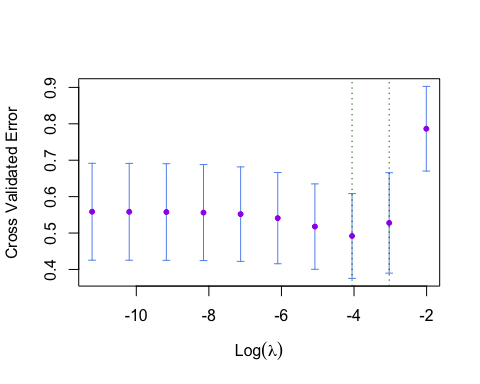
\includegraphics{Reproducibility_Bayesian_Regression_of_Directional_Data_MarkDown_files/figure-latex/unnamed-chunk-4-1.pdf}

\begin{Shaded}
\begin{Highlighting}[]
\NormalTok{  Posterior\_mean}\OtherTok{=}\FunctionTok{apply}\NormalTok{(lst}\SpecialCharTok{$}\NormalTok{MC}\SpecialCharTok{$}\NormalTok{Mc\_Beta, }\AttributeTok{MARGIN =} \FunctionTok{c}\NormalTok{(}\DecValTok{2}\NormalTok{,}\DecValTok{3}\NormalTok{), }\AttributeTok{FUN =}\NormalTok{ mean)}
\NormalTok{  Posterior\_SD}\OtherTok{=}\FunctionTok{apply}\NormalTok{(lst}\SpecialCharTok{$}\NormalTok{MC}\SpecialCharTok{$}\NormalTok{Mc\_Beta, }\AttributeTok{MARGIN =} \FunctionTok{c}\NormalTok{(}\DecValTok{2}\NormalTok{,}\DecValTok{3}\NormalTok{), }\AttributeTok{FUN =}\NormalTok{ sd)}
  \FunctionTok{print}\NormalTok{(}\FunctionTok{cbind}\NormalTok{(}\AttributeTok{Posterior\_mean=}\FunctionTok{c}\NormalTok{(}\FunctionTok{t}\NormalTok{(Posterior\_mean)),}\AttributeTok{TrueValue=}\FunctionTok{c}\NormalTok{(}\FunctionTok{t}\NormalTok{(data\_lst}\SpecialCharTok{$}\NormalTok{beta))))}
\end{Highlighting}
\end{Shaded}

\begin{verbatim}
##       Posterior_mean  TrueValue
##  [1,]      9.1433008  9.1780961
##  [2,]      8.1409968  8.6681013
##  [3,]     -0.6898688 -0.6367181
##  [4,]      0.9126806  1.0669862
##  [5,]     -1.0447018 -0.9401547
##  [6,]      2.9017440  3.1512520
##  [7,]    -10.0534820 -9.9057587
##  [8,]      7.8050178  7.6063437
##  [9,]      6.9451379  7.4608627
## [10,]      2.3622122  2.7716209
## [11,]      3.3773247  3.5646314
## [12,]      6.7440190  6.9443400
## [13,]      1.8938526  1.6829277
## [14,]     -4.6336103 -4.7351207
## [15,]     -3.7336603 -3.4959589
## [16,]      8.8120898  9.3280394
## [17,]     -8.6656657 -8.4068649
## [18,]      3.5185716  3.4663838
## [19,]     -2.4707769 -2.2482709
## [20,]     -6.2764192 -6.5462095
\end{verbatim}

\hypertarget{simulated-data-generation-and-em-for-posterior-mode-d3-spherical-data}{%
\subsection{Simulated Data Generation and EM for Posterior Mode (d=3,
Spherical
Data):}\label{simulated-data-generation-and-em-for-posterior-mode-d3-spherical-data}}

In this part of the demonstration, we generate a dataset of size n=750,
with p=10 (10 covariates) and the responses are circular,i.e., d=2. Then
we fit the EM algorithm to estimate the regression coefficients. True
value of the regression coefficients, and its estimates are printed.

\begin{Shaded}
\begin{Highlighting}[]
\NormalTok{n}\OtherTok{=}\DecValTok{750}  \CommentTok{\# NUmber of the samples}
\NormalTok{p}\OtherTok{=}\DecValTok{10}    \CommentTok{\# NUmber of the regression covariates}
\NormalTok{d}\OtherTok{=}\DecValTok{3}     \CommentTok{\# Number of direcions in the direcional data}
\DocumentationTok{\#\#\#\# bbeta is a matrix of dimension p\textbackslash{}times d}
\CommentTok{\#bbeta=matrix( rnorm(p*d), nrow=p, ncol=d)}
\NormalTok{sigma\_square}\OtherTok{=}\DecValTok{1}
\NormalTok{tau\_square}\OtherTok{=}\DecValTok{10000}
\NormalTok{data\_lst }\OtherTok{=} \FunctionTok{Data\_generator\_vnf\_reg}\NormalTok{(}\AttributeTok{n=}\NormalTok{n, }\AttributeTok{p=}\NormalTok{p, }\AttributeTok{d=}\NormalTok{d, }\AttributeTok{concentration\_factor =} \DecValTok{1}\NormalTok{, }\AttributeTok{beta\_factor =} \DecValTok{10}\NormalTok{)}
\NormalTok{Y }\OtherTok{=}\NormalTok{ data\_lst}\SpecialCharTok{$}\NormalTok{Y;X}\OtherTok{=}\NormalTok{data\_lst}\SpecialCharTok{$}\NormalTok{X;}

\CommentTok{\# Fitting the EM algorithm for the Standard Regresion for directional responses: This takes less than a minute. }
\NormalTok{beta\_EM}\OtherTok{=}\FunctionTok{EM\_Dir\_regression\_optimizer\_V1}\NormalTok{(}\AttributeTok{Y=}\NormalTok{Y, }\AttributeTok{X=}\NormalTok{X, }\AttributeTok{prior=}\ConstantTok{NULL}\NormalTok{, }\AttributeTok{beta\_init =} \ConstantTok{NULL}\NormalTok{,   }\AttributeTok{EM\_tolerence =}\NormalTok{ .}\DecValTok{00001}\NormalTok{)}
\end{Highlighting}
\end{Shaded}

\begin{verbatim}
## [1] 2
## [1] 3
## [1] 4
## [1] 5
## [1] 6
## [1] 7
## [1] 8
## [1] 9
## [1] 10
## [1] 11
## [1] 12
## [1] 13
## [1] 14
## [1] 15
## [1] 16
## [1] 17
## [1] 18
## [1] 19
## [1] 20
## [1] 21
## [1] 22
## [1] 23
## [1] 24
## [1] 25
## [1] 26
## [1] 27
## [1] 28
## [1] 29
## [1] 30
## [1] 31
## [1] 32
## [1] 33
## [1] 34
## [1] 35
## [1] 36
## [1] 37
## [1] 38
## [1] 39
## [1] 40
## [1] 41
## [1] 42
## [1] 43
## [1] 44
## [1] 45
## [1] 46
## [1] 47
## [1] 48
## [1] 49
## [1] 50
## [1] 51
## [1] 52
## [1] 53
## [1] 54
## [1] 55
## [1] 56
## [1] 57
## [1] 58
## [1] 59
## [1] 60
## [1] 61
## [1] 62
## [1] 63
## [1] 64
## [1] 65
## [1] 66
## [1] 67
## [1] 68
## [1] 69
## [1] 70
## [1] 71
## [1] 72
## [1] 73
## [1] 74
## [1] 75
## [1] 76
## [1] 77
## [1] 78
## [1] 79
## [1] 80
## [1] 81
## [1] 82
## [1] 83
## [1] 84
## [1] 85
## [1] 86
## [1] 87
## [1] 88
## [1] 89
## [1] 90
## [1] 91
## [1] 92
## [1] 93
## [1] 94
## [1] 95
## [1] 96
## [1] 97
## [1] 98
## [1] 99
## [1] 100
## [1] 101
## [1] 102
## [1] 103
## [1] 104
## [1] 105
## [1] 106
## [1] 107
## [1] 108
## [1] 109
## [1] 110
## [1] 111
## [1] 112
## [1] 113
## [1] 114
## [1] 115
## [1] 116
## [1] 117
## [1] 118
## [1] 119
## [1] 120
## [1] 121
## [1] 122
## [1] 123
## [1] 124
## [1] 125
## [1] 126
## [1] 127
## [1] 128
## [1] 129
## [1] 130
## [1] 131
## [1] 132
## [1] 133
## [1] 134
## [1] 135
## [1] 136
## [1] 137
## [1] 138
## [1] 139
## [1] 140
## [1] 141
## [1] 142
## [1] 143
## [1] 144
## [1] 145
## [1] 146
## [1] 147
## [1] 148
## [1] 149
## [1] 150
## [1] 151
## [1] 152
## [1] 153
## [1] 154
## [1] 155
## [1] 156
## [1] 157
## [1] 158
## [1] 159
## [1] 160
## [1] 161
## [1] 162
## [1] 163
## [1] 164
## [1] 165
## [1] 166
## [1] 167
## [1] 168
## [1] 169
## [1] 170
## [1] 171
## [1] 172
## [1] 173
## [1] 174
## [1] 175
## [1] 176
## [1] 177
## [1] 178
## [1] 179
## [1] 180
## [1] 181
## [1] 182
## [1] 183
## [1] 184
## [1] 185
## [1] 186
## [1] 187
## [1] 188
## [1] 189
## [1] 190
## [1] 191
## [1] 192
## [1] 193
## [1] 194
## [1] 195
## [1] 196
## [1] 197
## [1] 198
## [1] 199
## [1] 200
## [1] 201
## [1] 202
## [1] 203
## [1] 204
## [1] 205
## [1] 206
## [1] 207
## [1] 208
## [1] 209
## [1] 210
## [1] 211
## [1] 212
## [1] 213
## [1] 214
## [1] 215
## [1] 216
## [1] 217
## [1] 218
## [1] 219
## [1] 220
## [1] 221
## [1] 222
## [1] 223
## [1] 224
## [1] 225
## [1] 226
## [1] 227
## [1] 228
## [1] 229
## [1] 230
## [1] 231
## [1] 232
## [1] 233
## [1] 234
## [1] 235
## [1] 236
## [1] 237
## [1] 238
## [1] 239
## [1] 240
## [1] 241
## [1] 242
## [1] 243
## [1] 244
## [1] 245
## [1] 246
## [1] 247
## [1] 248
## [1] 249
## [1] 250
## [1] 251
## [1] 252
## [1] 253
## [1] 254
## [1] 255
## [1] 256
## [1] 257
## [1] 258
## [1] 259
## [1] 260
## [1] 261
## [1] 262
## [1] 263
## [1] 264
## [1] 265
## [1] 266
## [1] 267
## [1] 268
## [1] 269
## [1] 270
## [1] 271
## [1] 272
## [1] 273
## [1] 274
## [1] 275
## [1] 276
## [1] 277
## [1] 278
\end{verbatim}

\begin{Shaded}
\begin{Highlighting}[]
\FunctionTok{colnames}\NormalTok{(beta\_EM)}\OtherTok{=} \FunctionTok{gsub}\NormalTok{(}\StringTok{"Y"}\NormalTok{,}\StringTok{"Beta"}\NormalTok{, }\FunctionTok{colnames}\NormalTok{(beta\_EM))}
\FunctionTok{print}\NormalTok{(beta\_EM)}
\end{Highlighting}
\end{Shaded}

\begin{verbatim}
##           Beta_1     Beta_2    Beta_3
##  [1,] -5.1204582  9.4532879  6.693824
##  [2,] -7.6044770 -2.8252978  9.359304
##  [3,]  0.5676267 -6.7663135  3.524529
##  [4,] -8.6822086 -0.1843894 -3.757477
##  [5,]  5.4379897  2.1709632 -5.098061
##  [6,]  0.4489144  4.5622368  0.381783
##  [7,] -9.0411462  9.3852345 -3.842344
##  [8,] -6.5778652  0.9028781 -7.554037
##  [9,]  0.8758519 -1.0354903  7.417748
## [10,]  2.6219600  6.8012298  3.585278
\end{verbatim}

\begin{Shaded}
\begin{Highlighting}[]
\FunctionTok{print}\NormalTok{(}\FunctionTok{cbind}\NormalTok{(}\AttributeTok{EstimatedValue=}\FunctionTok{c}\NormalTok{(}\FunctionTok{t}\NormalTok{(beta\_EM)),}\AttributeTok{TrueValue=}\FunctionTok{c}\NormalTok{(}\FunctionTok{t}\NormalTok{(data\_lst}\SpecialCharTok{$}\NormalTok{beta))))}
\end{Highlighting}
\end{Shaded}

\begin{verbatim}
##       EstimatedValue  TrueValue
##  [1,]     -5.1204582 -5.1032424
##  [2,]      9.4532879  9.2202933
##  [3,]      6.6938239  6.6520589
##  [4,]     -7.6044770 -7.6079044
##  [5,]     -2.8252978 -2.9394490
##  [6,]      9.3593036  9.1576316
##  [7,]      0.5676267  0.6041939
##  [8,]     -6.7663135 -6.7932816
##  [9,]      3.5245289  3.8252544
## [10,]     -8.6822086 -8.5716502
## [11,]     -0.1843894 -0.4964653
## [12,]     -3.7574768 -3.8573423
## [13,]      5.4379897  5.5753166
## [14,]      2.1709632  2.5198880
## [15,]     -5.0980611 -5.4439783
## [16,]      0.4489144  0.3591816
## [17,]      4.5622368  4.6959955
## [18,]      0.3817830 -0.4615122
## [19,]     -9.0411462 -9.1170453
## [20,]      9.3852345  9.1142326
## [21,]     -3.8423440 -3.7901064
## [22,]     -6.5778652 -6.5410895
## [23,]      0.9028781  0.9152809
## [24,]     -7.5540370 -7.4511749
## [25,]      0.8758519  1.1853333
## [26,]     -1.0354903 -1.1711221
## [27,]      7.4177483  7.1559290
## [28,]      2.6219600  2.6191717
## [29,]      6.8012298  6.9910047
## [30,]      3.5852785  3.5501845
\end{verbatim}

\hypertarget{bayesian-mcmc-algorithmd3}{%
\subsection{Bayesian MCMC
Algorithm(d=3):}\label{bayesian-mcmc-algorithmd3}}

Here we obtain the posterior samples of the regression coefficients
using the MCMC algorithm.

\begin{Shaded}
\begin{Highlighting}[]
\CommentTok{\# Change Sample Size to get the full MCMC. MCMC step takes time depending on the sample size. This step can take 20 to 30 minutes. Prints output after every 100 samples are generated.}
\NormalTok{lst}\OtherTok{=}\FunctionTok{MCMC\_Dir\_regression\_sampler\_V1}\NormalTok{(}\AttributeTok{Y=}\NormalTok{data\_lst}\SpecialCharTok{$}\NormalTok{Y, }\AttributeTok{X=}\NormalTok{data\_lst}\SpecialCharTok{$}\NormalTok{X, }\AttributeTok{prior=}\ConstantTok{NULL}\NormalTok{, }\AttributeTok{beta\_init =} \ConstantTok{NULL}\NormalTok{, }\AttributeTok{MCSamplerSize =}\DecValTok{100}\NormalTok{)}
\end{Highlighting}
\end{Shaded}

\begin{verbatim}
## [1] "Default Procedure using EM is being used to obtain initial value of the regression coefficients that will be  used to start the MCMC Data Augmentation Algorithm. Iteration number of EM algorithm is being printed untill convergence."
## [1] 2
## [1] 3
## [1] 4
## [1] 5
## [1] 6
## [1] 7
## [1] 8
## [1] 9
## [1] 10
## [1] 11
## [1] 12
## [1] 13
## [1] 14
## [1] 15
## [1] 16
## [1] 17
## [1] 18
## [1] 19
## [1] 20
## [1] 21
## [1] 22
## [1] 23
## [1] 24
## [1] 25
## [1] 26
## [1] 27
## [1] 28
## [1] 29
## [1] 30
## [1] 31
## [1] 32
## [1] 33
## [1] 34
## [1] 35
## [1] 36
## [1] 37
## [1] 38
## [1] 39
## [1] 40
## [1] 41
## [1] 42
## [1] 43
## [1] 44
## [1] 45
## [1] 46
## [1] 47
## [1] 48
## [1] 49
## [1] 50
## [1] 51
## [1] 52
## [1] 53
## [1] 54
## [1] 55
## [1] 56
## [1] 57
## [1] 58
## [1] 59
## [1] 60
## [1] 61
## [1] 62
## [1] 63
## [1] 64
## [1] 65
## [1] 66
## [1] 67
## [1] 68
## [1] 69
## [1] 70
## [1] 71
## [1] 72
## [1] 73
## [1] 74
## [1] 75
## [1] 76
## [1] 77
## [1] 78
## [1] 79
## [1] 80
## [1] 81
## [1] 82
## [1] 83
## [1] 84
## [1] 85
## [1] 86
## [1] 87
## [1] 88
## [1] 89
## [1] 90
## [1] 91
## [1] 92
## [1] 93
## [1] 94
## [1] 95
## [1] 96
## [1] 97
## [1] 98
## [1] 99
## [1] 100
## [1] 101
## [1] 102
## [1] 103
## [1] 104
## [1] 105
## [1] 106
## [1] 107
## [1] 108
## [1] 109
## [1] 110
## [1] 111
## [1] 112
## [1] 113
## [1] 114
## [1] 115
## [1] 116
## [1] 117
## [1] 118
## [1] 119
## [1] 120
## [1] 121
## [1] 122
## [1] 123
## [1] 124
## [1] 125
## [1] 126
## [1] 127
## [1] 128
## [1] 129
## [1] 130
## [1] 131
## [1] 132
## [1] 133
## [1] 134
## [1] 135
## [1] 136
## [1] 137
## [1] 138
## [1] 139
## [1] 140
## [1] 141
## [1] 142
## [1] 143
## [1] 144
## [1] 145
## [1] 146
## [1] 147
## [1] 148
## [1] 149
## [1] 150
## [1] 151
## [1] 152
## [1] 153
## [1] 154
## [1] 155
## [1] 156
## [1] 157
## [1] 158
## [1] 159
## [1] 160
## [1] 161
## [1] 162
## [1] 163
## [1] 164
## [1] 165
## [1] 166
## [1] 167
## [1] 168
## [1] 169
## [1] 170
## [1] 171
## [1] 172
## [1] 173
## [1] 174
## [1] 175
## [1] 176
## [1] 177
## [1] 178
## [1] 179
## [1] 180
## [1] 181
## [1] 182
## [1] 183
## [1] 184
## [1] 185
## [1] 186
## [1] 187
## [1] 188
## [1] 189
## [1] 190
## [1] 191
## [1] 192
## [1] 193
## [1] 194
## [1] 195
## [1] 196
## [1] 197
## [1] 198
## [1] 199
## [1] 200
## [1] 201
## [1] 202
## [1] 203
## [1] 204
## [1] 205
## [1] 206
## [1] 207
## [1] 208
## [1] 209
## [1] 210
## [1] 211
## [1] 212
## [1] 213
## [1] 214
## [1] 215
## [1] 216
## [1] 217
## [1] 218
## [1] 219
## [1] 220
## [1] 221
## [1] 222
## [1] 223
## [1] 224
## [1] 225
## [1] 226
## [1] 227
## [1] 228
## [1] 229
## [1] 230
## [1] 231
## [1] 232
## [1] 233
## [1] 234
## [1] 235
## [1] 236
## [1] 237
## [1] 238
## [1] 239
## [1] 240
## [1] 241
## [1] 242
## [1] 243
## [1] 244
## [1] 245
## [1] 246
## [1] 247
## [1] 248
## [1] 249
## [1] 250
## [1] 251
## [1] 252
## [1] 253
## [1] 254
## [1] 255
## [1] 256
## [1] 257
## [1] 258
## [1] 259
## [1] 260
## [1] 261
## [1] 262
## [1] 263
## [1] 264
## [1] 265
## [1] 266
## [1] 267
## [1] 268
## [1] 269
## [1] 270
## [1] 271
## [1] 272
## [1] 273
## [1] 274
## [1] 275
## [1] 276
## [1] 277
## [1] 278
## [1] " Initial value and prior information obtained successfully.  The MCMC samples are being generated. This step may take significnt amount of time depending on the MCMC sample size to be Generated.   "
## [1] "MC_Iter=100completed"
\end{verbatim}

The triplet plot (autocorrelation, traceplot and density plot) for some
of the regression coefficient is plotted (d=3)

\begin{Shaded}
\begin{Highlighting}[]
\CommentTok{\# Summary from MCMC output}
\NormalTok{i}\OtherTok{=}\DecValTok{1}\NormalTok{;j}\OtherTok{=} \DecValTok{1}
  \FunctionTok{Plot\_MCMC\_Diag\_Triplet}\NormalTok{(lst}\SpecialCharTok{$}\NormalTok{MC}\SpecialCharTok{$}\NormalTok{Mc\_Beta[,i,j],}\AttributeTok{y\_lab\_text =} \FunctionTok{bquote}\NormalTok{(beta[.(i)][.(j)]))}
\end{Highlighting}
\end{Shaded}

\includegraphics{Reproducibility_Bayesian_Regression_of_Directional_Data_MarkDown_files/figure-latex/unnamed-chunk-7-1.pdf}

\begin{Shaded}
\begin{Highlighting}[]
\NormalTok{  Posterior\_mean}\OtherTok{=}\FunctionTok{apply}\NormalTok{(lst}\SpecialCharTok{$}\NormalTok{MC}\SpecialCharTok{$}\NormalTok{Mc\_Beta, }\AttributeTok{MARGIN =} \FunctionTok{c}\NormalTok{(}\DecValTok{2}\NormalTok{,}\DecValTok{3}\NormalTok{), }\AttributeTok{FUN =}\NormalTok{ mean)}
\NormalTok{  Posterior\_SD}\OtherTok{=}\FunctionTok{apply}\NormalTok{( lst}\SpecialCharTok{$}\NormalTok{MC}\SpecialCharTok{$}\NormalTok{Mc\_Beta, }\AttributeTok{MARGIN =} \FunctionTok{c}\NormalTok{(}\DecValTok{2}\NormalTok{,}\DecValTok{3}\NormalTok{), }\AttributeTok{FUN =}\NormalTok{ sd)}
  \FunctionTok{print}\NormalTok{(}\FunctionTok{cbind}\NormalTok{(}\AttributeTok{Posterior\_mean=}\FunctionTok{c}\NormalTok{(}\FunctionTok{t}\NormalTok{(Posterior\_mean)),}\AttributeTok{TrueValue=}\FunctionTok{c}\NormalTok{(}\FunctionTok{t}\NormalTok{(data\_lst}\SpecialCharTok{$}\NormalTok{beta))))}
\end{Highlighting}
\end{Shaded}

\begin{verbatim}
##       Posterior_mean  TrueValue
##  [1,]     -5.0417465 -5.1032424
##  [2,]      9.4058652  9.2202933
##  [3,]      6.6019410  6.6520589
##  [4,]     -7.5419220 -7.6079044
##  [5,]     -2.7867454 -2.9394490
##  [6,]      9.2772396  9.1576316
##  [7,]      0.5710165  0.6041939
##  [8,]     -6.6835783 -6.7932816
##  [9,]      3.4687574  3.8252544
## [10,]     -8.6300589 -8.5716502
## [11,]     -0.1737290 -0.4964653
## [12,]     -3.7007190 -3.8573423
## [13,]      5.3914242  5.5753166
## [14,]      2.1210339  2.5198880
## [15,]     -5.0628199 -5.4439783
## [16,]      0.4715700  0.3591816
## [17,]      4.5514895  4.6959955
## [18,]      0.3804979 -0.4615122
## [19,]     -8.9220565 -9.1170453
## [20,]      9.3131514  9.1142326
## [21,]     -3.8299039 -3.7901064
## [22,]     -6.5047913 -6.5410895
## [23,]      0.8556865  0.9152809
## [24,]     -7.4736338 -7.4511749
## [25,]      0.8474118  1.1853333
## [26,]     -1.0290243 -1.1711221
## [27,]      7.3002311  7.1559290
## [28,]      2.5807921  2.6191717
## [29,]      6.7166005  6.9910047
## [30,]      3.5725952  3.5501845
\end{verbatim}

\hypertarget{simulated-data-generation-and-em-for-posterior-mode-d10-higher-dimensional-spherical-data}{%
\subsection{Simulated Data Generation and EM for Posterior Mode (d=10,
Higher dimensional Spherical
Data):}\label{simulated-data-generation-and-em-for-posterior-mode-d10-higher-dimensional-spherical-data}}

In this part of the demonstration, we generate a dataset of size n=750,
with p=10 (10 covariates) and the responses are circular,i.e., d=2. Then
we fit the EM algorithm to estimate the regression coefficients. True
value of the regression coefficients, and its estimates are printed.

\begin{Shaded}
\begin{Highlighting}[]
\NormalTok{n}\OtherTok{=}\DecValTok{750}  \CommentTok{\# NUmber of the samples}
\NormalTok{p}\OtherTok{=}\DecValTok{10}    \CommentTok{\# NUmber of the regression covariates}
\NormalTok{d}\OtherTok{=}\DecValTok{10}     \CommentTok{\# Number of direcions in the direcional data}
\DocumentationTok{\#\#\#\# bbeta is a matrix of dimension p\textbackslash{}times d}
\CommentTok{\#bbeta=matrix( rnorm(p*d), nrow=p, ncol=d)}
\NormalTok{sigma\_square}\OtherTok{=}\DecValTok{1}
\NormalTok{tau\_square}\OtherTok{=}\DecValTok{10000}
\NormalTok{data\_lst }\OtherTok{=} \FunctionTok{Data\_generator\_vnf\_reg}\NormalTok{(}\AttributeTok{n=}\NormalTok{n, }\AttributeTok{p=}\NormalTok{p, }\AttributeTok{d=}\NormalTok{d, }\AttributeTok{concentration\_factor =} \DecValTok{1}\NormalTok{, }\AttributeTok{beta\_factor =} \DecValTok{10}\NormalTok{)}
\NormalTok{Y }\OtherTok{=}\NormalTok{ data\_lst}\SpecialCharTok{$}\NormalTok{Y;X}\OtherTok{=}\NormalTok{data\_lst}\SpecialCharTok{$}\NormalTok{X;}

\CommentTok{\# Fitting the EM algorithm for the Standard Regresion for directional responses: This takes less than a minute. }
\NormalTok{beta\_EM}\OtherTok{=}\FunctionTok{EM\_Dir\_regression\_optimizer\_V1}\NormalTok{(}\AttributeTok{Y=}\NormalTok{Y, }\AttributeTok{X=}\NormalTok{X, }\AttributeTok{prior=}\ConstantTok{NULL}\NormalTok{, }\AttributeTok{beta\_init =} \ConstantTok{NULL}\NormalTok{,   }\AttributeTok{EM\_tolerence =}\NormalTok{ .}\DecValTok{00001}\NormalTok{)}
\end{Highlighting}
\end{Shaded}

\begin{verbatim}
## [1] 2
## [1] 3
## [1] 4
## [1] 5
## [1] 6
## [1] 7
## [1] 8
## [1] 9
## [1] 10
## [1] 11
## [1] 12
## [1] 13
## [1] 14
## [1] 15
## [1] 16
## [1] 17
## [1] 18
## [1] 19
## [1] 20
## [1] 21
## [1] 22
## [1] 23
## [1] 24
## [1] 25
## [1] 26
## [1] 27
## [1] 28
## [1] 29
## [1] 30
## [1] 31
## [1] 32
## [1] 33
## [1] 34
## [1] 35
## [1] 36
## [1] 37
## [1] 38
## [1] 39
## [1] 40
## [1] 41
## [1] 42
## [1] 43
## [1] 44
## [1] 45
## [1] 46
## [1] 47
## [1] 48
## [1] 49
## [1] 50
## [1] 51
## [1] 52
## [1] 53
## [1] 54
## [1] 55
## [1] 56
## [1] 57
## [1] 58
## [1] 59
## [1] 60
## [1] 61
## [1] 62
## [1] 63
## [1] 64
## [1] 65
## [1] 66
## [1] 67
## [1] 68
## [1] 69
## [1] 70
## [1] 71
## [1] 72
## [1] 73
## [1] 74
## [1] 75
## [1] 76
## [1] 77
## [1] 78
## [1] 79
## [1] 80
## [1] 81
## [1] 82
## [1] 83
## [1] 84
## [1] 85
## [1] 86
## [1] 87
## [1] 88
## [1] 89
## [1] 90
## [1] 91
## [1] 92
## [1] 93
## [1] 94
## [1] 95
## [1] 96
## [1] 97
## [1] 98
## [1] 99
## [1] 100
## [1] 101
## [1] 102
## [1] 103
## [1] 104
## [1] 105
## [1] 106
## [1] 107
## [1] 108
## [1] 109
## [1] 110
## [1] 111
## [1] 112
## [1] 113
## [1] 114
## [1] 115
## [1] 116
## [1] 117
## [1] 118
## [1] 119
## [1] 120
## [1] 121
## [1] 122
## [1] 123
\end{verbatim}

\begin{Shaded}
\begin{Highlighting}[]
\FunctionTok{colnames}\NormalTok{(beta\_EM)}\OtherTok{=} \FunctionTok{gsub}\NormalTok{(}\StringTok{"Y"}\NormalTok{,}\StringTok{"Beta"}\NormalTok{, }\FunctionTok{colnames}\NormalTok{(beta\_EM))}
\FunctionTok{print}\NormalTok{(beta\_EM)}
\end{Highlighting}
\end{Shaded}

\begin{verbatim}
##           Beta_1    Beta_2    Beta_3     Beta_4     Beta_5    Beta_6     Beta_7
##  [1,]  7.3992823  5.876836  4.771418 -8.1093643  0.3444737  4.524083 -3.2393136
##  [2,]  0.5319963  9.725552 -0.626292  0.3549782 -0.4688477 -2.122460 -2.6516922
##  [3,]  6.2617098 -7.408357  2.315447 -0.7419082 -3.9174655 -5.075964 -6.1855462
##  [4,] -6.7154488  4.022847  2.755982  1.6993616 -2.4595542 -3.643728 -8.8778996
##  [5,] -3.5533861 -0.210946  1.412101  1.7004054  0.8907576  3.183308  9.8722996
##  [6,]  5.2224384  8.826334  0.456063  4.6789345  6.7215937 -2.687346  4.6746693
##  [7,] -1.5449089  8.679246 -3.346191  2.9491693  6.2435251 -8.152633  0.4182507
##  [8,]  3.4955450 -6.092324 -1.609596  4.7735288  0.9805911  6.749988 -4.0447465
##  [9,]  3.9770705 -6.820566  4.234451 -8.6822331  4.1576627 -6.193440  9.1187673
## [10,] -3.5713125 -4.808413  9.888930 -2.2874023 -6.4283902 -7.051818  8.7902379
##           Beta_8    Beta_9    Beta_10
##  [1,]  6.4006044  7.510263  2.8020400
##  [2,]  2.4252438  1.385517 -0.4535819
##  [3,] -9.9288982  6.082198 -0.6795813
##  [4,] -6.3124319  2.085605 -2.9552260
##  [5,]  7.7892587 -6.671992  1.3117033
##  [6,]  1.8876265 -9.828252 -8.1597713
##  [7,]  0.7829697 -6.931669 -2.4459499
##  [8,]  7.3687655 -7.860467 -0.5825884
##  [9,]  5.9774959  8.397092  0.5880563
## [10,]  1.3753778  4.764684  9.4117644
\end{verbatim}

\begin{Shaded}
\begin{Highlighting}[]
\FunctionTok{print}\NormalTok{(}\FunctionTok{cbind}\NormalTok{(}\AttributeTok{EstimatedValue=}\FunctionTok{c}\NormalTok{(}\FunctionTok{t}\NormalTok{(beta\_EM)),}\AttributeTok{TrueValue=}\FunctionTok{c}\NormalTok{(}\FunctionTok{t}\NormalTok{(data\_lst}\SpecialCharTok{$}\NormalTok{beta))))}
\end{Highlighting}
\end{Shaded}

\begin{verbatim}
##        EstimatedValue   TrueValue
##   [1,]      7.3992823  7.45396109
##   [2,]      5.8768361  5.70777595
##   [3,]      4.7714178  5.13479525
##   [4,]     -8.1093643 -8.34807107
##   [5,]      0.3444737 -0.11903854
##   [6,]      4.5240833  4.95393269
##   [7,]     -3.2393136 -2.72930281
##   [8,]      6.4006044  5.94673814
##   [9,]      7.5102629  7.26604964
##  [10,]      2.8020400  2.61417870
##  [11,]      0.5319963  0.02343572
##  [12,]      9.7255524  9.68971683
##  [13,]     -0.6262920 -0.83075497
##  [14,]      0.3549782  0.03072829
##  [15,]     -0.4688477 -0.80046967
##  [16,]     -2.1224596 -1.87904436
##  [17,]     -2.6516922 -2.80986251
##  [18,]      2.4252438  1.72185396
##  [19,]      1.3855173  1.99420214
##  [20,]     -0.4535819 -0.35861077
##  [21,]      6.2617098  6.22719322
##  [22,]     -7.4083569 -7.35675618
##  [23,]      2.3154473  1.77587852
##  [24,]     -0.7419082 -0.70855416
##  [25,]     -3.9174655 -3.58164667
##  [26,]     -5.0759637 -4.44560647
##  [27,]     -6.1855462 -6.11580417
##  [28,]     -9.9288982 -9.68276069
##  [29,]      6.0821980  5.72517364
##  [30,]     -0.6795813 -0.12569647
##  [31,]     -6.7154488 -6.63981815
##  [32,]      4.0228468  3.68955548
##  [33,]      2.7559815  2.76035415
##  [34,]      1.6993616  1.56297926
##  [35,]     -2.4595542 -2.49948581
##  [36,]     -3.6437280 -3.41236800
##  [37,]     -8.8778996 -8.71481293
##  [38,]     -6.3124319 -6.06268244
##  [39,]      2.0856049  1.78088282
##  [40,]     -2.9552260 -3.11674494
##  [41,]     -3.5533861 -3.46868088
##  [42,]     -0.2109460 -0.52491444
##  [43,]      1.4121010  1.88533348
##  [44,]      1.7004054  1.63546911
##  [45,]      0.8907576  0.95304366
##  [46,]      3.1833082  2.69289227
##  [47,]      9.8722996  9.68395981
##  [48,]      7.7892587  7.48289992
##  [49,]     -6.6719921 -6.82093495
##  [50,]      1.3117033  1.55465520
##  [51,]      5.2224384  5.10402876
##  [52,]      8.8263339  8.59148275
##  [53,]      0.4560630  0.44748847
##  [54,]      4.6789345  4.16967609
##  [55,]      6.7215937  6.76854962
##  [56,]     -2.6873460 -2.85553090
##  [57,]      4.6746693  4.44065592
##  [58,]      1.8876265  1.36772341
##  [59,]     -9.8282517 -9.74631346
##  [60,]     -8.1597713 -8.07965880
##  [61,]     -1.5449089 -1.34643138
##  [62,]      8.6792457  8.62556585
##  [63,]     -3.3461909 -3.00504376
##  [64,]      2.9491693  2.42319306
##  [65,]      6.2435251  5.95926298
##  [66,]     -8.1526329 -8.26616540
##  [67,]      0.4182507  0.34690494
##  [68,]      0.7829697  0.57918826
##  [69,]     -6.9316689 -6.80424527
##  [70,]     -2.4459499 -2.19301486
##  [71,]      3.4955450  3.36181150
##  [72,]     -6.0923241 -6.34672307
##  [73,]     -1.6095959 -1.15922001
##  [74,]      4.7735288  4.88044756
##  [75,]      0.9805911  0.93800439
##  [76,]      6.7499876  6.30480058
##  [77,]     -4.0447465 -4.12704619
##  [78,]      7.3687655  7.53876752
##  [79,]     -7.8604666 -7.89182804
##  [80,]     -0.5825884 -0.98398733
##  [81,]      3.9770705  3.76220463
##  [82,]     -6.8205657 -7.11230112
##  [83,]      4.2344512  3.99320192
##  [84,]     -8.6822331 -8.43479905
##  [85,]      4.1576627  4.53634838
##  [86,]     -6.1934404 -5.98684761
##  [87,]      9.1187673  8.86227657
##  [88,]      5.9774959  6.19382267
##  [89,]      8.3970916  8.45354562
##  [90,]      0.5880563  0.57341915
##  [91,]     -3.5713125 -3.39240250
##  [92,]     -4.8084127 -4.63635968
##  [93,]      9.8889299  9.79232684
##  [94,]     -2.2874023 -1.90586139
##  [95,]     -6.4283902 -6.79139737
##  [96,]     -7.0518176 -6.86485402
##  [97,]      8.7902379  8.74967757
##  [98,]      1.3753778  1.11962155
##  [99,]      4.7646841  4.77577786
## [100,]      9.4117644  9.27148033
\end{verbatim}

\hypertarget{bayesian-mcmc-algorithmd10}{%
\subsection{Bayesian MCMC
Algorithm(d=10):}\label{bayesian-mcmc-algorithmd10}}

Here we obtain the posterior samples of the regression coefficients
using the MCMC algorithm.

\begin{Shaded}
\begin{Highlighting}[]
\CommentTok{\# Change Sample Size to get the full MCMC. MCMC step takes time depending on the sample size. This step can take 20 to 30 minutes. Prints output after every 100 samples are generated.}
\NormalTok{lst}\OtherTok{=}\FunctionTok{MCMC\_Dir\_regression\_sampler\_V1}\NormalTok{(}\AttributeTok{Y=}\NormalTok{data\_lst}\SpecialCharTok{$}\NormalTok{Y, }\AttributeTok{X=}\NormalTok{data\_lst}\SpecialCharTok{$}\NormalTok{X, }\AttributeTok{prior=}\ConstantTok{NULL}\NormalTok{, }\AttributeTok{beta\_init =} \ConstantTok{NULL}\NormalTok{, }\AttributeTok{MCSamplerSize =}\DecValTok{100}\NormalTok{)}
\end{Highlighting}
\end{Shaded}

\begin{verbatim}
## [1] "Default Procedure using EM is being used to obtain initial value of the regression coefficients that will be  used to start the MCMC Data Augmentation Algorithm. Iteration number of EM algorithm is being printed untill convergence."
## [1] 2
## [1] 3
## [1] 4
## [1] 5
## [1] 6
## [1] 7
## [1] 8
## [1] 9
## [1] 10
## [1] 11
## [1] 12
## [1] 13
## [1] 14
## [1] 15
## [1] 16
## [1] 17
## [1] 18
## [1] 19
## [1] 20
## [1] 21
## [1] 22
## [1] 23
## [1] 24
## [1] 25
## [1] 26
## [1] 27
## [1] 28
## [1] 29
## [1] 30
## [1] 31
## [1] 32
## [1] 33
## [1] 34
## [1] 35
## [1] 36
## [1] 37
## [1] 38
## [1] 39
## [1] 40
## [1] 41
## [1] 42
## [1] 43
## [1] 44
## [1] 45
## [1] 46
## [1] 47
## [1] 48
## [1] 49
## [1] 50
## [1] 51
## [1] 52
## [1] 53
## [1] 54
## [1] 55
## [1] 56
## [1] 57
## [1] 58
## [1] 59
## [1] 60
## [1] 61
## [1] 62
## [1] 63
## [1] 64
## [1] 65
## [1] 66
## [1] 67
## [1] 68
## [1] 69
## [1] 70
## [1] 71
## [1] 72
## [1] 73
## [1] 74
## [1] 75
## [1] 76
## [1] 77
## [1] 78
## [1] 79
## [1] 80
## [1] 81
## [1] 82
## [1] 83
## [1] 84
## [1] 85
## [1] 86
## [1] 87
## [1] 88
## [1] 89
## [1] 90
## [1] 91
## [1] 92
## [1] 93
## [1] 94
## [1] 95
## [1] 96
## [1] 97
## [1] 98
## [1] 99
## [1] 100
## [1] 101
## [1] 102
## [1] 103
## [1] 104
## [1] 105
## [1] 106
## [1] 107
## [1] 108
## [1] 109
## [1] 110
## [1] 111
## [1] 112
## [1] 113
## [1] 114
## [1] 115
## [1] 116
## [1] 117
## [1] 118
## [1] 119
## [1] 120
## [1] 121
## [1] 122
## [1] 123
## [1] " Initial value and prior information obtained successfully.  The MCMC samples are being generated. This step may take significnt amount of time depending on the MCMC sample size to be Generated.   "
## [1] "MC_Iter=100completed"
\end{verbatim}

The triplet plot (autocorrelation, traceplot and density plot) for some
of the regression coefficient is plotted (d=10)

\begin{Shaded}
\begin{Highlighting}[]
\CommentTok{\# Summary from MCMC output}
\NormalTok{i}\OtherTok{=}\DecValTok{1}\NormalTok{;j}\OtherTok{=} \DecValTok{1}
  \FunctionTok{Plot\_MCMC\_Diag\_Triplet}\NormalTok{(lst}\SpecialCharTok{$}\NormalTok{MC}\SpecialCharTok{$}\NormalTok{Mc\_Beta[,i,j],}\AttributeTok{y\_lab\_text =} \FunctionTok{bquote}\NormalTok{(beta[.(i)][.(j)]))}
\end{Highlighting}
\end{Shaded}

\includegraphics{Reproducibility_Bayesian_Regression_of_Directional_Data_MarkDown_files/figure-latex/unnamed-chunk-10-1.pdf}

\begin{Shaded}
\begin{Highlighting}[]
\NormalTok{  Posterior\_Mean}\OtherTok{=}\FunctionTok{apply}\NormalTok{(lst}\SpecialCharTok{$}\NormalTok{MC}\SpecialCharTok{$}\NormalTok{Mc\_Beta, }\AttributeTok{MARGIN =} \FunctionTok{c}\NormalTok{(}\DecValTok{2}\NormalTok{,}\DecValTok{3}\NormalTok{), }\AttributeTok{FUN =}\NormalTok{ mean)}
\NormalTok{  Posterior\_SD}\OtherTok{=}\FunctionTok{apply}\NormalTok{( lst}\SpecialCharTok{$}\NormalTok{MC}\SpecialCharTok{$}\NormalTok{Mc\_Beta, }\AttributeTok{MARGIN =} \FunctionTok{c}\NormalTok{(}\DecValTok{2}\NormalTok{,}\DecValTok{3}\NormalTok{), }\AttributeTok{FUN =}\NormalTok{ sd)}
  \FunctionTok{print}\NormalTok{(}\FunctionTok{cbind}\NormalTok{(}\AttributeTok{Estimated\_Value=}\FunctionTok{c}\NormalTok{(}\FunctionTok{t}\NormalTok{(Posterior\_Mean)),}\AttributeTok{TrueValue=}\FunctionTok{c}\NormalTok{(}\FunctionTok{t}\NormalTok{(data\_lst}\SpecialCharTok{$}\NormalTok{beta))))}
\end{Highlighting}
\end{Shaded}

\begin{verbatim}
##        Estimated_Value   TrueValue
##   [1,]       7.4675023  7.45396109
##   [2,]       5.9375361  5.70777595
##   [3,]       4.8748452  5.13479525
##   [4,]      -8.2569558 -8.34807107
##   [5,]       0.3198340 -0.11903854
##   [6,]       4.6160452  4.95393269
##   [7,]      -3.2823731 -2.72930281
##   [8,]       6.5324955  5.94673814
##   [9,]       7.6198506  7.26604964
##  [10,]       2.8829515  2.61417870
##  [11,]       0.4974261  0.02343572
##  [12,]       9.8750824  9.68971683
##  [13,]      -0.6776207 -0.83075497
##  [14,]       0.3254709  0.03072829
##  [15,]      -0.4362816 -0.80046967
##  [16,]      -2.1651889 -1.87904436
##  [17,]      -2.7052221 -2.80986251
##  [18,]       2.4733492  1.72185396
##  [19,]       1.3813091  1.99420214
##  [20,]      -0.4886024 -0.35861077
##  [21,]       6.3699931  6.22719322
##  [22,]      -7.5551533 -7.35675618
##  [23,]       2.3719635  1.77587852
##  [24,]      -0.7892019 -0.70855416
##  [25,]      -4.0400511 -3.58164667
##  [26,]      -5.1410863 -4.44560647
##  [27,]      -6.2711171 -6.11580417
##  [28,]     -10.1425130 -9.68276069
##  [29,]       6.1466760  5.72517364
##  [30,]      -0.7573701 -0.12569647
##  [31,]      -6.7972541 -6.63981815
##  [32,]       4.0946718  3.68955548
##  [33,]       2.7805033  2.76035415
##  [34,]       1.7149174  1.56297926
##  [35,]      -2.4447050 -2.49948581
##  [36,]      -3.7188972 -3.41236800
##  [37,]      -9.0030460 -8.71481293
##  [38,]      -6.4139092 -6.06268244
##  [39,]       2.1118924  1.78088282
##  [40,]      -2.9674371 -3.11674494
##  [41,]      -3.6081631 -3.46868088
##  [42,]      -0.1980248 -0.52491444
##  [43,]       1.4582715  1.88533348
##  [44,]       1.7578694  1.63546911
##  [45,]       0.9118947  0.95304366
##  [46,]       3.2872134  2.69289227
##  [47,]      10.0231568  9.68395981
##  [48,]       7.8842844  7.48289992
##  [49,]      -6.8070288 -6.82093495
##  [50,]       1.2759593  1.55465520
##  [51,]       5.2998675  5.10402876
##  [52,]       8.9909418  8.59148275
##  [53,]       0.4335566  0.44748847
##  [54,]       4.7777307  4.16967609
##  [55,]       6.8373735  6.76854962
##  [56,]      -2.7263003 -2.85553090
##  [57,]       4.7370537  4.44065592
##  [58,]       1.9211992  1.36772341
##  [59,]      -9.9763173 -9.74631346
##  [60,]      -8.3420029 -8.07965880
##  [61,]      -1.5479066 -1.34643138
##  [62,]       8.8910917  8.62556585
##  [63,]      -3.4226740 -3.00504376
##  [64,]       2.9866824  2.42319306
##  [65,]       6.3468206  5.95926298
##  [66,]      -8.2856701 -8.26616540
##  [67,]       0.4070208  0.34690494
##  [68,]       0.7738870  0.57918826
##  [69,]      -7.1095458 -6.80424527
##  [70,]      -2.4995880 -2.19301486
##  [71,]       3.5396073  3.36181150
##  [72,]      -6.1865192 -6.34672307
##  [73,]      -1.5554162 -1.15922001
##  [74,]       4.8579113  4.88044756
##  [75,]       1.0516862  0.93800439
##  [76,]       6.8361600  6.30480058
##  [77,]      -4.1010856 -4.12704619
##  [78,]       7.5137582  7.53876752
##  [79,]      -7.9785727 -7.89182804
##  [80,]      -0.6005667 -0.98398733
##  [81,]       4.0395719  3.76220463
##  [82,]      -6.8947066 -7.11230112
##  [83,]       4.2897081  3.99320192
##  [84,]      -8.8464776 -8.43479905
##  [85,]       4.2382118  4.53634838
##  [86,]      -6.3434542 -5.98684761
##  [87,]       9.2863745  8.86227657
##  [88,]       6.1090241  6.19382267
##  [89,]       8.5391887  8.45354562
##  [90,]       0.6058325  0.57341915
##  [91,]      -3.6317465 -3.39240250
##  [92,]      -4.9265329 -4.63635968
##  [93,]      10.0585232  9.79232684
##  [94,]      -2.3344698 -1.90586139
##  [95,]      -6.5595411 -6.79139737
##  [96,]      -7.1720910 -6.86485402
##  [97,]       8.9438268  8.74967757
##  [98,]       1.3956960  1.11962155
##  [99,]       4.8710395  4.77577786
## [100,]       9.5578973  9.27148033
\end{verbatim}

\end{document}
